\setchapterpreamble[u]{\margintoc}
\chapter{Общие сведения теории формальных языков}
\label{chpt:FormalLanguageTheoryIntro}
\tikzsetfigurename{FormalLanguageTheoryIntro_}

В данной главе мы рассмотрим основные понятия из теории формальных языков, которые пригодятся нам в дальнейшем изложении.
Заметим, что мы рассмотрим лишь те результаты теории формальных языков,которые будут необходимы нам для дальнейшего изложения.
Для более глубокого изучения именно теории формальных языков рекомендуется обратиться к классической литературе.
Например, к работам Харрисона~\cite{10.5555/578595}, Хопкрофта~\cite{hopcroft2001introduction} или другой подобной литературе.
\marginnote[*2]{
    В рамках данной работы мы будем говорить о \enquote{типичных} языках, элементами которых являются объекты, максимально похожие на строки.
    При этом будет оставлен за бортом тот факт, что базовое определение позволяет нам рассматривать в качестве \enquote{строительных элементов} (алфавита) практически произвольные объекты, а значит, создавать весьма нетривиальные конструкции в качестве слов языка.
    Примерами \enquote{нестроковых} языков могут послужить языки деревьев~\cite{tata2007} или языки графов~\cite{EHRIG1992557, Courcelle2009}.
}

\begin{definition}[Алфавит]
    \emph{Алфавит}~--- это конечное множество.
    Элементы этого множества будем называть \emph{символами}.
\end{definition}

\begin{example}
    Примеры алфавитов.
    \begin{itemize}
        \item Латинский алфавит $\Sigma = \{a, b, c, \dots, z\}$.
        \item Кириллический алфавит $\Sigma = \{\text{а, б, в, \dots, я}\}$.
        \item Алфавит натуральных чисел в шестнадцатеричной записи
              \[\Sigma = \{0, 1, 2, 3, 4, 5, 6, 7 ,8, 9, A, B, C, D, E, F\}.\]
    \end{itemize}
\end{example}

Традиционное обозначение для алфавита~--- $\Sigma$.
Также мы будем использовать различные прописные буквы латинского алфавита.
Для обозначения символов алфавита будем использовать строчные буквы латинского алфавита: $a, b, \dots, x, y, z$.

Будем считать, что над алфавитом $\Sigma$ всегда определена операция конкатенации $\cdot: \Sigma^* \times \Sigma^* \to \Sigma^*$.
\marginnote{TODO: объяснить звездочку Клини}
При записи выражений символ точки (обозначение операции конкатенации) часто будем опускать: $a \cdot b = ab$.

\begin{definition}[Слово]
    \emph{Слово} над алфавитом $\Sigma$~--- это конечная конкатенация символов алфавита $\Sigma$: $\omega = a_0 \cdot a_1 \cdot \dots \cdot a_m$, где $\omega$~--- слово, а $a_i \in \Sigma$ для любого $i$.
    Для обозначения пустого слова (слова, содержащего ноль символов) будем использовать специальный символ $\varepsilon, \varepsilon \notin \Sigma$.
\end{definition}

\begin{definition}[Длина слова]
    Пусть $\omega = a_0 \cdot a_1 \cdot \dots \cdot a_m$~--- слово над алфавитом $\Sigma$.
    Будем называть $m + 1$ \emph{длиной слова} и обозначать как $|\omega|$.
    Длина пустого слова равна нулю.
\end{definition}

\begin{definition}[Количество вхождений символа]
    Пусть $\omega$~--- слово над алфавитом $\Sigma$. Пусть $t \in \Sigma$~--- некоторый символ из алфавита.
    Тогда будем обозначать количество вхождений символа $t$ в слове $\omega$ как $|\omega|_t$.
\end{definition}

\begin{definition}[Язык]
    \emph{Язык} над алфавитом $\Sigma$~--- это множество слов над алфавитом $\Sigma$.
\end{definition}

\begin{example}
    Примеры языков.

    \begin{itemize}
        \item Язык целых чисел в двоичной записи $\{0, 1, -1, 10, 11, -10, -11, \dots\}$.
              \marginnote{TODO: Меня смущает - перед бинарными числами}
        \item Язык всех правильных скобочных последовательностей
              \[\{(), (()), ()(), (())(), \dots\}.\]
    \end{itemize}
\end{example}

Любой язык над алфавитом $\Sigma$ является подмножеством универсального множества $\Sigma^*$~--- множества всех слов над алфавитом $\Sigma$.

Заметим, что язык не обязан быть конечным множеством, в то время как алфавит в нашей области всегда конечен%
\sidenote{Существуют ситуации, когда возникают бесконечные алфавиты.}
и изучаем мы конечные слова%
\sidenote{
    Существуют ситуации, когда возникают бесконечные слова.
    Например работы по обработке потоков.
}.

Можно выделить следующие основные \emph{способы задания языков}.
\begin{itemize}
    \item Перечислить все элементы.
          Такой способ работает только для конечных языков.
          Перечислить бесконечное множество за конечное время не получится.
    \item Задать генератор~--- процедуру, которая возвращает очередное слово языка.
    \item Задать распознаватель~--- процедуру, которая по данному слову может определить, принадлежит оно заданному языку или нет.
\end{itemize}

Стоит отметить, что существуют и другие способы задания.
Например, язык может определяться как решение некоторого \emph{языкового уравнения}~\sidecite{Leiss1999}.

\section{Теоретико-множественные операции над языками}

Так как язык~--- это \emph{множество} слов, то над языками естественным образом определены теоретико-множественные операции, такие как объединение, пересечение, дополнение.
\begin{itemize}
    \item $L_1 \cup L_2 = \{ \omega \mid \omega \in L_1 \text{ или } \omega \in L_2\}$
    \item $L_1 \cap L_2 = \{ \omega \mid \omega \in L_1 \text{ и } \omega \in L_2\}$
    \item $\overline{L} = \{ \omega \mid \omega \in \Sigma^* \text{ и } \omega \notin L\}$, где $L$~--- язык над алфавитом $\Sigma$ .
\end{itemize}

Но кроме этого, нам потребуются и относительно специальные операции, определённые ниже.

\begin{definition}[TODO: Что ты такое]
    Пусть дано множество $S$ с определённой на нём операцией $\odot: S \times S \to S$, $S_1 \subseteq S$, $S_2 \subseteq S$, тогда
    \[S_1 \odot S_2 = \{ s_1 \odot s_2 \mid s_1 \in S_1, s_2 \in S_2\}.\]
\end{definition}

\begin{definition}[TODO: ???]
    Пусть дано множество $S$ с определённой на нём операцией $\odot: S \times S \to S$, $S_1 \subseteq S$, тогда
    \[S_1^n = \{ \underbrace{s_1 \odot s_1 \odot \dots \odot s_1}_{\text{$n$ раз}} \mid s_1 \in S_1\}.\]
    При этом $S_1^0 = \{\varepsilon\}$%
    \sidenote{В данном случае нулевая степень даёт единицу, как мы и привыкли.}.
\end{definition}

\begin{definition}[TODO: ???]
    Пусть дано множество $S$ с определённой на нём операцией $\odot: S \times S \to S$, $S_1 \subseteq S$, тогда
    \[S_1^* = \bigcup_{n = 0}^{\infty} S_1^n.\]
\end{definition}

Многие прикладные задачи, в которых возникают языки, достаточно естественным образом формулируются в теоретико-множественных терминах.
Так, задача распознавания~--- это задача проверки принадлежности элемента множеству.
Далее мы рассмотрим прикладные задачи, решение которых требует, например, проверки включения одного языка в другой, или проверки непустоты пересечения двух языков.
Разрешимость таких задач, алгоритмы решения, их сложность и другие свойства, зависят от свойств языков.
Это даёт дополнительную связь теоретико-языковых конструкций с решением прикладных задач, позволяя более аккуратно рассуждать о свойствах получаемых решений.

\section{Производные}

Производные для языков предложил Януш Бжозовский в работе~\sidecite{10.1145/321239.321249}.

\begin{definition}[Производная Бжозовского]
    Производная $\partial_c L = \{ w' \mid w \in L, w = cw'\}$.
\end{definition}

Заметим, что если для слова $w$, $|w| = n$ верно, что
\[\varepsilon \in (\partial_{w[n-1]} \circ \dots \circ \partial_{w[1]}  \circ \partial_{w[0]}) (L),\]
то $w \in L$.
Таким образом, существует возможность использовать производные для проверки принадлежность слов заданному языку.
Данная возможность активно используется для регулярных языков~\sidecite{caron_champarnaud_mignot_2014}, языков, распознаваемых автоматами, управляемыми входом (Input Driven Pushdown Automata, IDPDA)~\sidecite{10.1145/3591472}, и контекстно-свободных языков~\sidecite{10.1145/2034773.2034801, 10.1145/3022671.2984026}.
Кроме этого, с помощью производных можно построить элегантный алгоритм построения конечного автомата по регулярному выражению~\sidecite{10.1017/S0956796808007090} и для выполнения регулярных запросов~\sidecite{10.1145/2949689.2949711}.

\section{Распознаватели}

Распознаватель может быть сконструирован как некоторая формальная машина, которая принимает или отвергает те или иные слова, записанные на входной ленте.
Таким образом, язык задаваемый некоторым вычислителем~--- это множество принимаемых им слов.
Далее становится возможно классифицировать языки по тому, какого класса распознаватель необходим и достаточен, чтобы их задать.
Например, можно выделить класс языков, задаваемых конечными автоматами.
На этом, в частности, построена \emph{иерархия Хомского}.

\section{Генераторы}

Один из базовых способов задать генератор языка опирается на \emph{системы переписывания строк}, из которых, в дальнейшем, можно получить так называемые \emph{порождающие грамматики}.

\begin{definition}[Система переписывания]
    \emph{Система переписывания (строк)}%
    \sidenote{Один из классически примеров систем переписывания строк~--- это машины Маркова, или алгорифмы Маркова~\cite{markov1954theory}.}~---
    это пара $R = \langle \Sigma, P  \rangle$, где $\Sigma$~--- алфавит, $P= \{p \mid p = w' \to w'', w' \in \Sigma^+, w'' \in \Sigma^*\}$~--- набор правил переписывания.
\end{definition}

Один шаг работы системы состоит из замены любого вхождения любой из левых частей правил на соответствующую правую часть правила.
Иными словами, пусть есть слово $w = w_0 w_1 w_2$ и имеется правило $w_1 \to w_3 \in P$.
Тогда после переписывания по этому правилу будет получено слово $w' = w_0 w_3 w_2$.
Заметим, что выбор заменяемого вхождения, как и выбор применяемого правила недетерминирован: может быть выбрано любое из вхождений и применено любое из доступных правил.
В качестве критерия остановки выберем невозможность применить ни одно из доступных правил.
Получившееся при этом слово будем считать результатом работы машины.
Зафиксировав стартовую строку и набор правил, можно достаточно естественным образом получить язык, как множество всех слов, являющихся результатом работы машины.

Представленная система является, скорее, неформальной базой для создания более содержательных систем.
Далее, накладывая дополнительные ограничения на правила машины и алгоритм её работы, мы будем получать некоторые содержательные классы языков.

Отметим, что подход к определению языков через системы переписывания не всегда удобен. Например, не получается с их использованием естественным образом определить булевы языки.

\section{Классы языков}

Иерархия языков, предложенная Ноамом Хомским (Noam Chomsky), является на текущий момент классической и представлена на рисунке~\ref{fig:Chomsky}.
Она основана на сопоставлении языкам тех или иных формальных вычислителей, способных их распознать.
Например, для распознавания любого регулярного языка достаточно конечного автомата. Для контекстно-свободного~--- магазинного автомата. И так далее.

\begin{figure}
    \caption{Иерархия языков по Хомскому}
    \label{fig:Chomsky}
    \begin{center}
        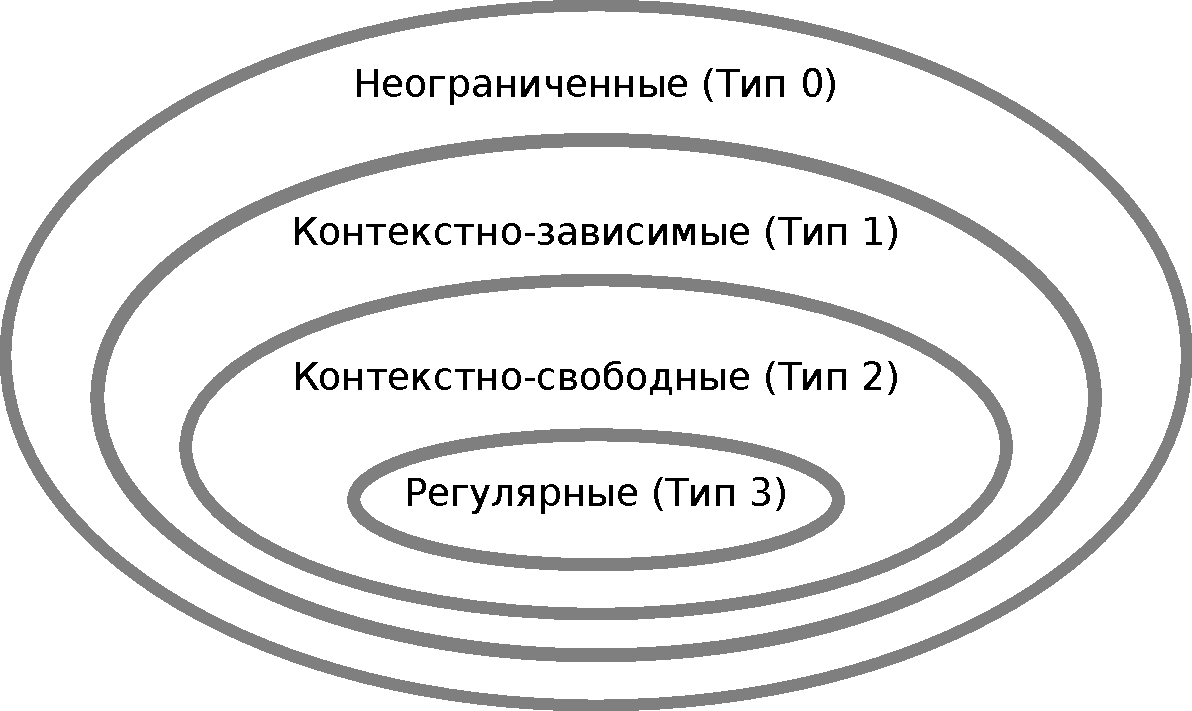
\includegraphics[width=0.9\textwidth]{figures/Chomsky.pdf}
    \end{center}
\end{figure}

Однако, данная иерархия постепенно теряет свою актуальность, так как появляются новые классы языков, свойства которых уже не удаётся адекватным образом отобразить, используя её.

Один из вариантов иерархии языков, более полно отображающий современное состояние дел, предложен Александром Охотиным%
\sidenote{
    Иерархия и некоторые отражаемые ей свойства подробно обсуждаются в презентации Александра Охотина \enquote{Underlying principles and recurring ideas of formal grammars} (\url{https://users.math-cs.spbu.ru/~okhotin/talks/grammars_lata_talk.pdf}).
    Также, с данной презентацией рекомендуется ознакомиться чтобы представить себе состояние области в целом.
}.
Вариация предложенной Александром Охотиным иерархии представлена на изображении~\ref{fig:hierarchyOkhotin}~
\sidenote{Данная вариация скомпонована из версии, представленной в презентации \enquote{Underlying principles and recurring ideas of formal grammars} и версии, взятой из работы~\cite{MRYKHIN2023113829}.}.
Приведённая диаграмма содержит регулярные и контекстно-свободные.
Так и подклассы, лежащие между ними.
Вместе с этим, классы, лежащие выше контекстно-свободных: многокомпонентные контекстно-свободные, булевы, конъюнктивные, их подклассы.

\begin{figure*}[h!]
    \caption{Иерархия. \emph{Reg}~--- регулярные, \emph{LLLin}, \emph{LRLin}, \emph{UnambLin}, \emph{Lin}, \emph{LL}, \emph{LR}, \emph{Unamb}~--- однозначные, \emph{Ordinary}~--- обыкновенные (контекстно-свободные)
        \emph{Conj}~--- конъюнктивные, \emph{Boolean}~--- булевы, \emph{UnamnbBool}, \emph{UnambConj}, \emph{VPDA}, \emph{LinConj}, \emph{UnambTAG}, \emph{TAG}, \emph{MCFL},}
    \label{fig:hierarchyOkhotin}
    \begin{center}
        \begin{tikzpicture}[node distance=1.0cm,bend angle=45,auto]
            \tikzstyle{lang}=[circle,thick,draw=blue!75,fill=blue!75,minimum size=1mm]
            \node [lang] (reg) [label=below:\emph{Reg}] {};
            \node [right of = reg] (reg_dummy) {};
            \node [lang] (lllin) [right of=reg_dummy, label=below:\emph{LLLin}] {};
            \node [right of = lllin] (lllin_dummy) {};
            \node [lang] (lrlin) [right of=lllin_dummy, label=below:\emph{LRLin}] {};
            \node [right of = lrlin] (lrlin_dummy) {};
            \node [lang] (unamblin) [right of=lrlin_dummy, label=below:\emph{UnambLin}] {};
            \node [right of = unamblin] (unamblin_dummy) {};
            \node [lang] (lin) [right of=unamblin_dummy, label=below:\emph{Lin}] {};
            \node [right of = lin] (lin_dummy) {};
            \node [right of = lin_dummy] (lin_dummy_2) {};
            \node [right of = lin_dummy_2] (lin_dummy_3) {};
            \node [lang] (conj) [right of=lin_dummy_3, label=below:\emph{Conj}] {};
            \node [right of = conj] (conj_dummy) {};
            \node [lang] (bool) [right of=conj_dummy, label=right:\emph{Bool}] {};

            \node [above of = lrlin] (lrlin_up_dummy) {};
            \node [lang] (ll) [above of=lrlin_up_dummy, label=above:\emph{LL}] {};
            \node [right of = ll] (ll_dummy) {};
            \node [lang] (lr) [right of=ll_dummy, label=above:\emph{LR}] {};
            \node [right of = lr] (lr_dummy) {};
            \node [lang] (unamb) [right of=lr_dummy, label=above:\emph{Unamb}] {};
            \node [right of = unamb] (unamb_dummy) {};
            \node [lang] (ordinary) [right of=unamb_dummy, label=right:\emph{Ordinary}] {};

            \node [lang] (conjleftcontext) [above of=conj_dummy, label=right:\emph{Conj$+\lhd$}] {};

            \node [below of = lrlin] (lrlin_down_dummy) {};
            \node [lang] (vpda) [below of=lrlin_down_dummy, label=below:\emph{VPDA}] {};
            \node [below of = lin] (lin_down_dummy_1) {};
            \node [below of = lin_down_dummy_1] (lin_down_dummy_2) {};
            \node [right of = lin_down_dummy_2] (lin_right_dummy_1) {};
            \node [lang] (linconj) [right of=lin_right_dummy_1, label=below:\emph{LinConj}] {};

            \node [lang] (unambtag) [above of=unamb_dummy, label=above:\emph{UnambTAG}] {};
            \node [right of = unambtag] (unambtag_dummy) {};
            \node [lang] (tag) [right of=unambtag_dummy, label=above:\emph{TAG}] {};
            \node [right of = tag] (tag_dummy) {};
            \node [lang] (mcfl) [right of=tag_dummy, label=above:\emph{MCFL}] {};

            \node [above of = linconj] (linconj_above_dummy) {};
            \node [lang] (unambconj) [right of=linconj_above_dummy, label=below:\emph{UnambConj}] {};
            \node [right of = unambconj] (unambconj_dummy) {};
            \node [lang] (unambbool) [right of=unambconj_dummy, label=right:\emph{UnambBool}] {};

            \node [below of = linconj] (linconj_below_dummy) {};
            \node [lang] (rtca) [right of=linconj_below_dummy, label=below:\emph{RT-CA}] {};
            \node [right of = rtca] (rtca_dummy) {};
            \node [lang] (ltca) [right of=rtca_dummy, label=right:\emph{LT-CA}] {};

            \path[->]
            (reg) edge node {} (lllin)
            (lllin) edge node {} (lrlin)
            (lrlin) edge node {} (unamblin)
            (unamblin) edge node {} (lin)

            (lllin) edge node {} (ll)
            (ll) edge node {} (lr)
            (ll) edge node {} (lr)
            (lr) edge node {} (unamb)
            (unamb) edge node {} (ordinary)

            (lrlin) edge node {} (lr)
            (unamblin) edge node {} (unamb)
            (lin) edge node {} (ordinary)

            (reg) edge node {} (vpda)
            (vpda) edge node {} (lr)
            (vpda) edge node {} (linconj)

            (ordinary) edge node {} (conj)
            (conj) edge node {} (bool)
            (conj) edge node {} (conjleftcontext)

            (unamb) edge node {} (unambtag)
            (ordinary) edge node {} (tag)
            (unambtag) edge node {} (tag)
            (tag) edge node {} (mcfl)

            (lin) edge node {} (linconj)
            (linconj) edge node {} (unambconj)
            (unambconj) edge node {} (unambbool)
            (unambconj) edge node {} (conj)
            (unambbool) edge node {} (bool)
            (unamb) edge node {} (unambconj)

            (linconj) edge node {} (rtca)
            (rtca) edge node {} (ltca)
            ;
        \end{tikzpicture}
    \end{center}
\end{figure*}

Для того, чтобы содержательно рассуждать про различные классы языков, необходимо иметь механизм, позволяющий чётко отделить один класс от другого.
\emph{Лемма о накачке} для соответствующего класса~--- один из классических таких механизмов.
Однако, не для всех классов языков соответствующие результаты получены.
Так, например, формулировка леммы о накачки для многокомпонентных контекстно-свободных языков в общем виде всё ещё не найдена, хотя существуют формулировки для отдельных подклассов.
Аналогично, для булевых и конъюнктивных языков всё ещё не предложены аналоги лемм о накачке.


%\section{Вопросы и задачи}
%\begin{enumerate}
%  \item !!!
%  \item !!!
%\end{enumerate}
